\documentclass[14pt]{extarticle}

\let\Overrightarrow\overrightarrow
\let\vecarrow\overrightarrow

%other%
\usepackage{graphicx}
\usepackage{float}
\usepackage[margin=0.7in]{geometry}
\usepackage{caption}
\usepackage{csquotes}
\usepackage[export]{adjustbox}
\usepackage{wrapfig}
\usepackage{setspace}
\usepackage{anyfontsize}
\usepackage{titlesec}
\titleformat{\section}{\normalfont\fontsize{20}{20}\bfseries}{\thesection}{1em}{}
\titleformat{\subsection}{\normalfont\fontsize{17}{20}\bfseries}{\thesubsection}{0.1em}{}
\usepackage{relsize}
\usepackage{indentfirst}
\usepackage{lipsum}
\usepackage{fancybox,framed}
\usepackage{comment}
\usepackage{enumitem}
\usepackage{biolinum}
%other%


%math%
\usepackage[fleqn]{amsmath}
\usepackage{amsthm}
\usepackage{nccmath}
\usepackage{amsmath}
\usepackage{amssymb}
\usepackage{mathtools}
\usepackage{yfonts}
%\usepackage{BOONDOX}

\usepackage{unicode-math}
\setmathfont{Latin Modern Math}

%\usepackage{unicode-math}
%\newtheorem*{}{\textup{Лемма}}
\newtheoremstyle{definition}
{3pt}
{3pt}
{\upshape}
{}
{\itshape\bfseries\fontsize{15}{15}}
{.}
{.5em}
{}
\theoremstyle{definition}
\newtheorem*{definition}{Определение}


%\newtheorem*{theorem}{\normalfont\fontsize{15}{15}\textup{Теорема}}
\newtheoremstyle{theorem}
{3pt}
{3pt}
{\itshape}
{}
{\bfseries\upshape\fontsize{15}{15}}
{.}
{.5em}
{}
%{\thmname{#1}\thmnumber{ #2}\thmnote{ (#3)}}

\usepackage{tikz}
   \usetikzlibrary{calc}

\newcommand{\arc}[0]{
   \tikz [baseline = (N.base), every node/.style={}] {
	  \node [inner sep = 0pt] (N){}; %{$#0$};
      \draw [line width = 0.8pt] plot [smooth, tension=1.3] coordinates {
         ($(N.north west) + (-1.5ex,0.6ex+0.4ex)$)
         ($(N.north)      + (-0.75ex,0+0.4ex)$)
         ($(N.north east) + (0ex,0.6ex+0.4ex)$)
      };
   }
}


\newcommand{\theoremmark} {
\tikz [baseline = (N.base), roundnode/.style={inner sep = 3pt, circle, draw=black!90, 
fill=white, very thick, minimum size=5mm},] {
\node [roundnode] (N){Т}    
    }
}


\theoremstyle{theorem}
\newtheorem*{theorem}{\theoremmark Теорема}

%\newcommand

%\newtheorem*{named}{\innerheader}

\newenvironment{namedtheorem}[2]
{
\newcommand{\foo}{#1}
\newtheorem*{\foo{}}{\normalfont\fontsize{15}{15}{\theoremmark Теорема #2}}
\begin{\foo{}}
}
{\end{\foo{}}}

%\newtheoremstyle{named}{}{}{\itshape}{}{\bfseries}{.}{.5em}{\thmnote{#3's}#1}
%\theoremstyle{named}
%\newtheorem*{namedtheorem}{theorem}
\newtheorem*{remark}{\textup{Комментарий}}
%\renewcommand\qedsymbol{$\blacksquare$}
%\usepackage{parski}
\renewenvironment{proof}
    {\noindent \textit{Доказательство.}\\
	\indent $\square$}
	{ $\blacksquare$\\ }

\newenvironment{solution}
	{\noindent\textbf{Решение.}}


\renewenvironment{remark}
    {\noindent\textbf{Комментарий.}}

\newenvironment{note}
    {\noindent {\normalfont\fontsize{14}{14}\textbf{\textit{Примечание.}}}}



\renewenvironment{rcases}
  {\left.\begin{aligned}}
  {\end{aligned}\right\rbrace}

\DeclarePairedDelimiter\abs{\lvert}{\rvert}
\DeclarePairedDelimiter\norm{\lVert}{\rVert}


%\newcounter{example}[section]
\newenvironment{example}[1]{\noindent \textbf{Пример #1.}}
%\newcommand{\mathleft}{\mathindent0pt}
%{\@fleqntrue}
%\@mathmargin0pt}
%math%

%fonts%
\usepackage[russian]{babel}
\usepackage{polyglossia}
\setdefaultlanguage[spelling=modern]{russian}
%\setotherlanguage{english}
\setmainfont{CMU Serif}
\setsansfont{CMU Sans Serif}
\setmonofont{CMU Typewriter Text}  
%\setmathfont{Latin Modern Math}

%\usepackage{fontspec}

%fonts%


\begin{document}


\begin{center}
%\centering
	\textbf{\fontsize{23}{30}\selectfont Конкурентные прямые.}
\end{center}

%В этом разделе мы рассмотрим одну из самых встречающихся тем 
%в олимпиадной геометрии (планиметрии). Это целый класс
%задач, в которых требуется доказать, что какие-то
%прямые пересекаются в одной точке (или параллельны), такие прямые ещё называют
%\textit{конкурентными}. Как правило их три, но может быть и больше.
%В данном разделе мы ограничимся рассмотрением примеров,
%где в основном фигурируют только три прямые.\\

В этом разделе мы рассмотрим целый класс
задач, в которых требуется доказать, что какие-то
прямые пересекаются в одной точке (или параллельны), такие прямые ещё называют
\textit{конкурентными}. Как правило их три, но может быть сколько угодно.
В данном разделе мы ограничимся рассмотрением примеров,
где \textit{в основном} фигурируют только три прямые.\\


\section*{Методы решения задач}

\subsection{Метод масс}
Для начала введем несколько базовых понятий и обозначений, которыми 
мы в дальнейшем будем пользоваться.\\

{\normalfont\fontsize{16}{16} \noindent \textbf{Обозначения}}

%[label={}, 
\begin{itemize}[leftmargin=*]

\item \(A(m)\) --- точка \(A\), которой сопоставлена масса \(m\).

\item \(\mathfrak{M}\) 
\footnote{{\fontsize{12}{12} \(\mathfrak{M}\) 
\textup{читается как \textit{\textquote{эм готическая}}}}}
= \(\big\{A_1(m_1), \, A_2(m_2), \dots , A_n(m_n) \big\}\) --- 
система матриальных точек,
состоящая из \(A_1(m_1), \, A_2(m_2), \dots , \, A_n(m_n)\).\\
Отметим, что так как \(\mathfrak{M}\) --- множество, то оно не
может содержать одинаковые элементы. А значит, если 
\(A_i = A_j (i \neq j)\), предварительно заменим их одной точкой,
например, \(A_i(m_i + m_j)\), где \(m_i\) и \(m_j\) --- 
массы в точках \(A_i\) и \(A_j\) соответственно. 

\item Запись \(Z = C(\mathfrak{M})\) будет обозначать, что 
\textit{центр масс} системы \(\mathfrak{M}\) существует и находится в \(Z\).
Иногда мы будем писать напрямую: \(Z = C(A_1, A_2, \dots , A_n)\), 
считая что массы \(m_1, m_2, \dots , m_n\), находящиеся в точках 
\(A_1, A_2, \dots , A_n\) соответственно, заранее оговорены.
%что будет означать, что \(Z\) -- центр масс системы материальных точек 
%\(A_1, A_2, \dots , A_n\).

%\item \(M(A(m), Z)\) --- момент материальной точки относительно точки \(Z\).

\end{itemize}

%\textbf{ТУТ БУДУТ ОБОЗНАЧЕНИЯ}

\begin{definition}
\noindent \textbf{Материальная точка} --- точка, которой 
\textit{приписана} некоторая масса.
\end{definition}

\begin{definition}
\noindent \textbf{Моментом} материальной точки $A(m)$ относительно 
точки $Z$ называют вектор $m \Overrightarrow{ZA_{\,}}$.
\end{definition}

\begin{definition}
\vspace{-3mm}
{\setstretch{1.7}
\noindent Точка $Z$ называется \textbf{центром масс} системы материальных 
точек $A_1(m_1), \, A_2(m_2), \dots , \, A_n(m_n)$, 
если $\mathlarger{\sum_{i=1}^{n} m_i \Overrightarrow{ZA_i} = \vecarrow{0_{\,}}}$.
\par}
\vspace{3mm}
\end{definition}



%\hspace{-8mm}
%\doublebox{
%\begin{minipage}{\textwidth - 6mm}
\begin{framed}
\noindent\textbf{\textit{Договоримся о следующем:}}
%\begin{enumerate}

%\item
Пусть имеется система материальных точек  
\(\mathfrak{M}\) и 
% = \big\{A_1(m_1), \, A_2(m_2),
%\, ... \, , \, A_n(m_n) \big\}\)
\(Z = C(\mathfrak{M})\).
%и \(\exists A_z(m_z) \in \mathfrak{M} \colon Z = A_z\). 
Тогда, говоря в дальнейшем о системе материальных точек
\(\mathfrak{M}\), % (возможно, опуская значок \(\mathfrak{M}\)),
мы будем подразумевать подсистему \(\mathfrak{M'}\), такую что 
\(\mathfrak{M'} = \big\{ A_i(m_i) \mid A_i(m_i) \in \mathfrak{M}, A_i \neq Z,
m_i \neq 0 \big\}\). 
%<То есть, мы просто убрали из \(\mathfrak{M}\) материальные точки,
%которые \textit{не влияют} на положение точки \(Z\) в пространстве.
%Однако нас, по сути, не интересует сама система, а интересует  
%только её центр масс. 
%Поскольку \(C(\mathfrak{M}) = C(\mathfrak{M'})\), то можно считать,
%что в рамках нашей теории \(\mathfrak{M} \thicksim \mathfrak{M'}\).>
%(Возможно, стоить убрать пояснение)
%
%\end{enumerate}
\end{framed} 
%\end{minipage}}\\
%\colon A_z(m_z) \notin
%\mathfrak{M'}, \, \forall A_i(m_i) \in \mathfrak{M'} \colon  A_i(m_i)
%\in \mathfrak{M}, \, m_i \neq 0 \}\). \\

%совпадает с одной из своих материальных точек,
%имеющих ненулевую массу, то будем вместо исходной системы считать 
%редуцированную систему, без этой точки. Иными словами, если 
%Договоримся о следующем: если 


В качестве физической интерпретации теории масс можно использовать
следующие соображения: \textbf{положительной} массе материальной точки \(m_1\)
сопоставить \textit{грузик} массы \(m_1\), а \textbf{отрицательной} массе 
\(m_2\) --- \textit{шарик} с соотвествующей подъемной силой,
по модулю равной силе тяжести, действующей на грузик массой \(|m_2|\).\\


\begin{theorem}[о существовании центра масс]
	Центр масс произвольной системы $A_1(m_1), \dots , A_n(m_n)$
	всегда существует, если $\mathlarger{\sum_{i=1}^{n} m_i \ne 0}$.
\end{theorem}

{\setstretch{1.8}
\begin{proof}
    Рассмотрим произвольную точку $X$. Тогда для любой  точки
	плоскости $O$ имеет место равенство $\mathlarger{\sum_{i=1}^{n}
	m_i  \Big(\vecarrow{XA_i} - \vecarrow{OX_{\, \,}}\Big) = \sum_{i=1}^{n} 
	m_i  \vecarrow{OA_i}}$. Тогда, чтобы точка $O$ была 
	центром масс системы, должно выполняться равенство
	$\mathlarger{\sum_{i=1}^{n} 
	m_i  \vecarrow{OA_i}} = \vecarrow{0_{\,}}$ $\iff \mathlarger{\sum_{i=1}^{n} m_i 
	\Big(\vecarrow{XA_i} - \vecarrow{OX_{\, \,}}\Big) = \vecarrow{0_{\,}} \iff 
    \vecarrow{XO_{\;}} = \frac{\displaystyle \sum \Big(m_i
	\vecarrow{XA_i} \Big)}{\displaystyle\sum m_i}}$. Таким образом, % \\\onehalfspacing\\ 
    утверждение о существовании \textit{центра масс} свелось к утверждению, что существует
	вектор $\vecarrow{XO_{\;}}$, заданный соответствующим соотношением, а он,
	понятное дело, существует.
\end{proof}
\par}

\begin{note}
	{\setstretch{2.0}
    Если условие $\mathlarger{\sum_{i=1}^{n} m_i \ne 0}$ не выполняется,
	то величина \\
	$\mathlarger{\abs*{\vecarrow{XO_{\;}}} = \frac{\displaystyle
    \abs*{\sum m_i \vecarrow{XA_i}}}{\displaystyle \sum m_i}}$
    не имеет смысла, поэтому это ограничение на сумму  масс %\\ \onehalfspacing 
    существенно. \par} \vspace{2mm}
    \noindent
    Физически объяснить отсутствие центра масс у системы материальных точек,
    сумма масс которой равна нулю, можно, например, следующим способом. \\
    От противного. Действительно, пусть имеется
    \(\mathfrak{M} = \big\{A_i(m_i) \mid i =
    1, \dots , n \big\}\), причем  \(\displaystyle \sum_{i = 1}^{n}
    m_i = 0\), \(Z = C(\mathfrak{M})\). 
    Пусть \(\mathfrak{M}_{A_1} = \mathfrak{M} \, \backslash \, 
    \{ A_1(m_1) \}\), \(B = C \left( \mathfrak{M}_{A_1}\right) \), 
    тогда система %\(\mathfrak{M}\)%сгруппируем все массы, за исключением
    \(A_1(m_1)\), \(B(-m_1)\) имеет ц.м. \(Z\) (по теореме о 
    группировке масс, см. далее). 
    Тогда, по определению центра масс,
    \(m_1 \vecarrow{ZA_1} + (-m_1) \vecarrow{ZB_{\, \,}} = 
    \vecarrow{0_{\,}} \iff A_1 = B\). 
    То есть \(A_1 = C \left( \mathfrak{M}_{A_1} \right)\), а значит 
    \(A_1 = C(\mathfrak{M})\), что противоречит договоренности, 
    описанной выше. Полученное противоречие завершает доказательство. \\
    

\end{note}

\begin{theorem}[о единственности центра масс]
    Если центр масс системы $A_1(m_1), A_2(m_2), \dots , A_n(m_n)$
	существует, то он единственен.
\end{theorem}

\begin{proof}
От противного. Пусть существуют два различных центра масс $Z$ и $Z'$.
Тогда по определению имеем: $\mathlarger{\sum_{i=1}^{n} m_i  \vecarrow{ZA_i}
= \vecarrow{0_{\,}},} \;  \mathlarger{\sum_{i=1}^{n} m_i  \vecarrow{Z'A_i}} = \vecarrow{0_{\,}}. 
\Rightarrow$ $\mathlarger{\sum_{i=1}^{n} m_i  \vecarrow{ZZ'_{\;\:\,}}} = \vecarrow{0_{\,}}$
$\iff \mathlarger{\vecarrow{ZZ'_{\;\:\,}} \sum_{i=1}^{n} m_i} = \vecarrow{0_{\,}}$. 
$\iff \vecarrow{ZZ'_{\;\:\,}} = \vecarrow{0_{\,}}$ (последний переход верен, 
так как центр масс существует, то есть
$\mathlarger{\sum_{i=1}^{n} m_i \ne 0}$) $\iff Z = Z'$, что противоречит
предположению, что точки $Z$ и $Z'$ различны. Следовательно,
центр масс $Z$ единственен, что и требовалось.
\end{proof}

\vspace{-3mm}
\begin{note}
Стоит отметить, что единственность мгновенно следует из единственности
вектора \(\vecarrow{XO_{\;}}\) (см. предыущее доказательство).\\
\end{note}


\noindent Далее будем считать, что $\mathlarger{\sum_{i=1}^{n} m_i \ne 0}$.

\begin{theorem}[о группировке масс]
Пусть есть система материальных точек $A_1(m_1), A_2(m_2), \dots ,
A_n(m_n), B_1(k_1), B_2(k_2), \dots , B_l(k_l)$, 
и подсистема $A_1(m_1), A_2(m_2), \dots , A_n(m_n)$ имеет центр масс 
$W\!.$ Назовем редуцированной системой систему $W(m_1 + ... + m_n), 
B_1(k_1), B_2(k_2), \dots , B_l(k_l)$. Тогда исходная система имеет 
ц.м. $Z$ в том и только том случае, когда редуцированная система 
имеет ц.м. $Z$.
\end{theorem}


%$\mathlarger{M = \sum_{i=1}^{l+n} m_i}$,\\
%$\mathlarger{A = \sum_{j=1}^{n} m_j}$.

\begin{proof}
Согласно \textit{определению} центра масс, надо доказать равносильность\\
$\mathlarger{\sum_{i=1}^{n} m_i \, \Overrightarrow{ZA_i} \: + 
\sum_{j=1}^{l} k_j \, \Overrightarrow{ZB_j}} = \vecarrow{0_{\,}} \iff 
\mathlarger{\sum_{j=1}^{l} k_j \, \Overrightarrow{ZB_j} + 
	 \sum_{i=1}^{n} m_i  \Overrightarrow{ZW_{\: \,}}} = \vecarrow{0_{\,}}$.
%\noindent 
То есть надо показать равенство:
$\mathlarger{\sum_{i=1}^{n} m_i \, \Overrightarrow{ZA_i} = 
\Overrightarrow{ZW_{\: \,}} \sum_{i=1}^{n} m_i}$ $\iff$   
$\mathlarger{\sum_{i=1}^{n}
m_i \, \Big(\Overrightarrow{ZA_i} - \Overrightarrow{ZW_{\: \,}}\Big)} = \vecarrow{0_{\,}}$ 
$\iff \mathlarger{\sum_{i=1}^{n}
m_i \, \Overrightarrow{WA_i}} = \vecarrow{0_{\,}}$, что верно в силу того, что $W$ ---
центр масс подсистемы $A_1(m_1), \, A_2(m_2), \, ... \, , \, A_n(m_n)$.
\end{proof}


Метод масс широко используется при доказательстве теорем и задач на
конкурентность прямых, причем их может быть любое количество, а ключевым 
элементом решения является именно \textit{теорема о группировке масс}.\\
Рассуждения могут выглядеть следующим образом:
\textit{\textquote{Докажем, что прямые \(x\), \(y\) и \(z\) пересекаются
в точке \(M\). Если нам удастся найти такие \(X \in x\), \(Y \in y\),
\(Z \in z\), что \(M = C(\mathfrak{M})\), где \(\mathfrak{M} =
\big\{X(m_x), 
Y(m_y), Z(m_z)\big\}\) для некоторых масс \(m_x, m_y, m_z\), 
\(C(X, Y) \in z\),
\(C(X, Z) \in y\),
\(C(Z, Y) \in x\),
то мы выполнили требуемое условие в силу \textbf{единственности} 
ц.м. \(M\).}}\\
А затем подбираются соответствующие точки \(X, Y, Z\) и соотвествующие 
массы \(m_x, m_y, m_z\).

\subsection{Теорема Чевы} 

\indent Один из самых мощных методов доказательства того, что три прямые 
проходят через одну точку или параллельны. 
Приведем ниже доказательство через \textit{метод масс}.
С другими доказательствами этой теоремы (через площадь, подобие и др.) 
вы можете ознакомится в других источниках, например, в книге Я. П. Понарина
\textquote{Элементарная геометрия. Том 1}.\\

\begin{namedtheorem}{ceva}{Чевы}
	Пусть на прямых $AB$, $BC$, $CA$, определяющих
    треугольник ABC, даны точки $C_1$, $A_1$, $B_1$. Для того, чтобы прямые
    $AA_1$, $BB_1$, $CC_1$ были конкурентны
    %пересекались в одной точке или были параллельными,
    необходимо и достаточно, чтобы
	
	\begin{ceqn}
	\[
    \dfrac{\Overrightarrow{AB_1}}{\Overrightarrow{B_1C_{\, \,}}} \cdot 
	\dfrac{\Overrightarrow{CA_1}}
	{\Overrightarrow{A_1B_{\:}}} \cdot \dfrac{\Overrightarrow{BC_1}}
	{\Overrightarrow{C_1A_{\,}}} = 1
	\]
    \end{ceqn}

\end{namedtheorem}


Мы же ограничемся лишь частным случаем данной теоремы, который используется 
чаще всего. А именно, когда точки \(A_1\), \(B_1\), \(C_1\) лежат на сторонах 
треугольника \(ABC\). С помощью метода масс можно доказать и общий вид данной 
теоремы, однако для этого придётся дополнительно разобрать несколько случаев, 
чего мы не будем делать, чтобы не усложнять восприятие самой идеи доказательства.\\ 

\begin{wrapfigure}{R}{9cm}
	\hspace{-0.3cm}
	%\vspace{-0.6cm}
	\vspace{-2cm}
	\fcolorbox{white}{white}{
		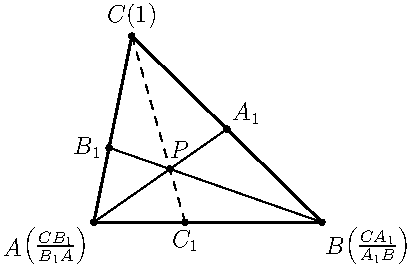
\includegraphics[width=9cm]{./img/theory/ceva.pdf}}
	\vspace{1cm}
\end{wrapfigure}

\begin{proof}
    Заметим, что существует ц.м. у \(\triangle ABC\) и у системы, 
    содержащей любые две вершины треугольника \(ABC\).
    %\textit{Необходимость.}
	Поместим массы \(1\), 
	\scalebox{0.8}{
    \hspace{-3.5mm}
    \(\dfrac{CA_1}{A_1B}\)},
    %
    \scalebox{0.8}{
    \hspace{-3.5mm}
    \(\dfrac{CB_1}{B_1A}\)}
    %
	в точки $C, \: B, \: A$ соответственно.
    
    Пусть \(BB_1 \cap AA_1 = P\). Тогда, по теореме о группировке масс, 
    \(C(A, B, C) \in BB_1\) (сгруппировали массы из точек \(A\) и \(C\) 
    в \(B_1\)) и \(C(A, B, C) \in AA_1\) (по той же причине). Следовательно, 
    \(P = C(A, B, C)\) в силу единственности центра масс. 
    Тогда \(P \in CC_1\) тогда и только тогда, когда 
    \(C_1 = C(A, B)\). А это, в свою очередь, равносильно тому, что 
    \(\dfrac{CB_1}{B_1A} \cdot \Overrightarrow{C_1A_{\,}} + 
      \dfrac{CA_1}{A_1B} \cdot \Overrightarrow{C_1B_{\:}} = \Overrightarrow{0_{\,}}\)
    \(\iff\)
    \(\dfrac{AB_1}{B_1C} \cdot \dfrac{CA_1}{A_1B} \cdot \dfrac{BC_1}{C_1A} = 1\).
    
    Полученное соотношение завершает доказательство, так как \(A_1\), \(B_1\), 
    \(C_1\) лежат на сторонах треугольника \(ABC\).
\end{proof}
%    
%    \scalebox{0.8}{
%    \hspace{-3.5mm}
%    \(\frac{\vphantom{A_{1_1}}
%    \Overrightarrow{\vphantom{AB'} CA_1}}{\vphantom
%	{\Overrightarrow{AB^{2'}}}\Overrightarrow{\vphantom{AB'}A_1B_{\, \,}}}
%    \)},
%    %\newline \noindent  
%    \scalebox{0.8}{
%    \hspace{-3.5mm}
%    \(\frac{\vphantom{A_{1_1}}
%    \Overrightarrow{\vphantom{AB'} CB_1}}{\vphantom
%	{\Overrightarrow{AB^{2'}}}\Overrightarrow{\vphantom{AB'}
%    B_1A_{\:}}}\)
%    }
    
%\(\frac{\overline{CB_1}}{\vphantom
    %{\overline{AB'}}\overline{B_1A}}\) (здесь за $\overline{v}$
	%обозначается вектор $v$)
   

%    Заметим, что существуют три случая:
%    \begin{enumerate}
%        \item Не существует ц. м. у треугольника \(ABC\).
%        \item Не существует ц. м. у точек \(B\) и \(C\).
%        \item Существуют оба из вышеописанных ц.м.
%    \end{enumerate} 


%    Сперва рассмотрим случай, когда ц.м. у треугольника \(ABC\)
%    не существует, то есть когда \(\dfrac{\Overrightarrow{CB_1}}
%	{\Overrightarrow{B_1A_{\,}}}  +
%	\dfrac{\Overrightarrow{CA_1}}{\Overrightarrow{A_1B_{\:}}} + 1 = 0\).
%    Докажем, что в этом и только в этом случае прямые \(AA_1\), \(BB_1\), 
%    \(CC_1\) параллельны.




%    Пусть теперь прямые  \(AA_1\), \(BB_1\), 
%    \(CC_1\) не все параллельны между собой, тогда положим
%     $AA_1 \cap BB_1 = P$. %, $CP \cap AB = C_1$. 
%    Тогда центр масс точек
%	$B$ и $C$ находится в $A_1$(он существует, так как сумма
%    масс в точках \(B\) и \(C\) никогда не бывает равна нулю),
%    а значит, сгруппировав массы из \(B\) и \(C\) в \(A_1\), получим, что 
%    %по \textit{теореме о
%    %группировке масс}, 
%    центр масс вершин $\triangle ABC$ лежит на
%    прямой $AA_1$ (центр масс двух точек лежит на прямой, содержащей эти точки).
%    Аналогично получаем, что он лежит и на $BB_1$.
%    Следовательно, $P$ --- центр масс вершин $\triangle ABC$, согласно 
%	\textit{теореме о единственности центра масс}. 
%	Так как $P \in CC_1$, то центр масс точек $B$ и $A$ находится в $C_1$
%    (если бы он был отличен от \(C_1\), то ц.м. \(\triangle ABC\)
%    лежал бы на прямой, проходящей через \(C\), и отличной от \(CC_1\), что 
%    противоречило бы единственности ц.м.).
%	Это равносильно тому, что $\dfrac{\Overrightarrow{CB_1}}
%	{\Overrightarrow{B_1A_{\,}}} \cdot \Overrightarrow{C_1A_{\,}} +
%	\Overrightarrow{C_1B_{\:}} \cdot
%	\dfrac{\Overrightarrow{CA_1}}{\Overrightarrow{A_1B_{\:}}} = \vecarrow{0_{\,}}$
%    $\iff$ 
%	$\dfrac{\Overrightarrow{AB_1}}{\Overrightarrow{B_1C_{\, \,}}} \cdot 
%	\dfrac{\Overrightarrow{CA_1}}
%	{\Overrightarrow{A_1B_{\:}}} \cdot \dfrac{\Overrightarrow{BC_1}}
%	{\Overrightarrow{C_1A_{\,}}} = 1$.
%    \vspace{1mm}
	

    %Пусть теперь  прямые $AA_1$ и $BB_1$ параллельны. Докажем, что 
	%тогда прямая $CC_1$ им параллельна. 
    %От противного. Пусть
	%$CC_1 \cap BB_1 = P$, тогда, аналогично доказанному выше, получаем, что
	%через точку $P$ проходит прямая $AA_1$, так как $P$ --- центр масс
	%вершин $\triangle ABC$, а мы доказали, что если две прямые
	%через него проходят, то и третья тоже через него проходит,
	%но $P \in BB_1$  противоречит предположению
	%$AA_1 \parallel BB_1. \implies CC_1 \parallel BB_1 \parallel AA_1$.\\
    %
    %\textit{Достаточность.}
    %
	%Мы доказали сразу и \textit{необходимость}, и \textit{достаточность},
	%потому что полученное выражение является критерием пренадлежности точки
	%$P$ прямой $CC_1$, то есть
	%того, что все три чевианы проходят через одну точку.
%\end{proof}

\begin{note}
%Как мы показали,
%\(AA_1 \parallel BB_1 \parallel CC_1\) равносильно тому, что у
%треугольника \(ABC\) с заданными массами не существует центра масс.\\ 
%К этому ещё можно относиться так: будем считать, что существует 
%\textit{бесконечно удаленная} прямая, содержащая \textit{бесконечно удаленные}
%точки, через каждую из которых проходит свое семейство параллельных прямых.
%Тогда, в случае, когда  \(AA_1 \parallel BB_1\), можно считать, что
%\(AA_1 \cap BB_1 = M\), где \(M\) --- бесконечно удаленная точка 
%(центр масс треугольника \(ABC\)). А так как
%\(M \in CC_1\) (см. случай, когда прямые непараллельны), 
%то \(AA_1 \parallel BB_1 \parallel CC_1\).
Формулу теоремы Чевы несложно запомнить, если при записи отношений
пользоваться правилом \textquote{\textit{в числителе: вектор от текущей вершины
до основания чевианы, для которого еще не записано отношение и которое лежит на 
прямой, содержащей вершину и сторону треугольника, 
а в знаменателе: вектор от текущего основания чевианы до другой вершины
на данной прямой}}.%, содержащей основание чевианы и предыдущую вершину
То есть мы обходим треугольник по или против часовой стрелки и записываем
отношения по данному правилу. Аналогичное правило применимо и к \textit{угловой}
теореме Чевы.\\
\end{note}
%$\blacksquare$ \\
%%\begin{remark}
%%\textup{
%%Доказательство остается верным, если точки $A_1, \: B_1, \: C_1$ лежат
%%так, что $AA_1 \parallel BB_1$, тогда ввиду следующих
%%соображений вышеописанные рассуждения остаются верными. Пусть $AA_1
%%\parallel BB_1$, тогда говорят, что $AA_1 \cap BB_1 = P$, где $P$ --- т.н. 
%%\textit{бесконечно удаленная точка}. Тогда вышеописанное тождество остается
%%критерием пренадлежности точки $P$ прямой $CC_1$, т.к. если $P \in CC_1$, то 
%%по определению \textit{бесконечно удаленной точки} --- $CC_1 \parallel BB_1
%%\parallel AA_1$, а если $CC_1 \nparallel AA_1$, то так же по определению
%%\textit{бесконечно удаленной точки} --- $P \notin CC_1$. %С геометрической же точки зрения это означает
%%}
%%\end{remark}


%\end{proof}



\noindent {\normalfont\fontsize{15}{15}\textbf{Дополнение}}


\begin{wrapfigure}{r}{7cm}
	\vspace{-1cm}
	\fcolorbox{white}{white}{
		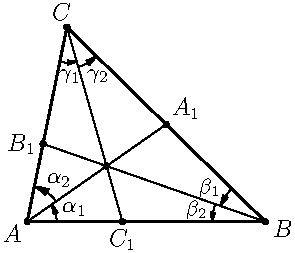
\includegraphics[width=6.5cm, left]{./img/theory/ceva_trig.pdf}}
	%\hspace{-5mm}
    
    %\hspace{1cm}	
%\vspace{-1.5cm}
\end{wrapfigure}

\noindent \textbf{\small Тригонометрическая (угловая) форма теоремы Чевы}.\\
Если ввести в рассмотрение \textit{ориентированные} углы $\alpha_1 = \angle BAA_1$, 
$\alpha_2 = \angle A_1AC$, $\gamma_1 = \angle ACC_1$, $\gamma_2 = \angle C_1CB$,
$\beta_1 = \angle CBB_1$, $\beta_2 = \angle B_1BA$, то соотношение теоремы
Чевы можно представить в эквивалентном виде через синусы этих углов, а именно


%\begin{flalign*}
{\setlength{\mathindent}{2.5cm}
\begin{equation*}
\dfrac{\sin \alpha_1}{\sin \alpha_2} \cdot 
	\dfrac{\sin \gamma_1}{\sin \gamma_2} 
\cdot \dfrac{\sin \beta_1}{\sin \beta_2} = 1 
\end{equation*}}
%\end{flalign*}
%\vspace{5mm}
	

    %\centerin

Предлагаем читателю доказать данное  утверждение самостоятельно, это 
будет хорошим упражнением.
%Если возникнут трудности, то можно обратиться к \textbf{примеру 1}, там есть
%соображения, которые могут помочь вам при доказательстве этой теоремы.

\subsection{Теорема Дезарга}
%\textbf{<ТУТ БУДЕТ ТЕОРЕМА ДЕЗАРГА>}\\
\begin{namedtheorem}{dezarg}{Дезарга}[обратная]
%Если существую точки пересечения 
Если точки пересечения прямых \(AB\) и \(A_1B_1\), \(BC\) и \(B_1C_1\), 
\(CA\) и \(C_1A_1\) лежат на одной прямой, то 
прямые \(AA_1\), \(BB_1\), \(CC_1\), соединяющие вершины треугольников 
\(ABC\) и \(A_1B_1C_1\), проходят через одну точку.
\end{namedtheorem}

Доказательство данного факта мы здесь приводить не будем, так как это выходит
за рамки данного раздела. Отметим только, что эту теорему можно доказать, 
например, с использованием теоремы Менелая или с помощью выхода в
пространство. С одним из них  вы можете ознакомиться самостоятельно, скажем,
в книге \textquote{Элементарная Геометрия Том 1}.
%С одним из них вы можете ознакомиться
%\newpage

\subsection{Принадлежность точки пересечения двух прямых третьей}

\begin{wrapfigure}{r}{7cm}

\vspace{0cm}
%\hspace{1cm}
%\centering
	\fcolorbox{white}{white}{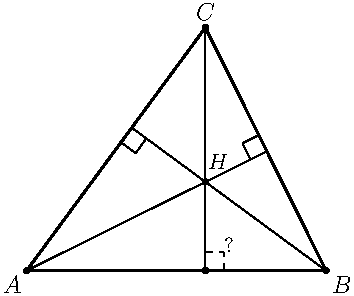
\includegraphics[width=7cm]{./img/theory/orthicproof.pdf}}
\vspace{-1cm}
\end{wrapfigure}

Можно попробовать доказать, что точка пересечения каких-то двух прямых из трех
принадлежит третьей. Классическим примером является доказательство
того, что \textit{высоты}, \textit{медианы}, \textit{серединные перпендикуляры} и
\textit{биссекрисы} треугольника пересекаются в одной точке.
С помощью данного метода иногда так же легко доказываются и более сложные вещи,
например, то, что \textit{радикальные оси} трех окружностей конкурентны. 
Точнее, таким способом можно доказать, что в \textit{нетривиальном} случае они 
проходят через одну точку, а \textit{тривиальный} случай можно разобрать
отдельно. Этот метод можно по-разному использовать, например, доказать
конкурентность высот треугольника можно исходя из следующих соображений: 
\textit{проведем две высоты и третью прямую, проходящую через точку пересечения
двух высот и через третью вершину треугольника, а потом докажем, что это и будет
искомая высота}.




\subsection{Преобразование плоскости}
Можно сделать \textit{преобразование плоскости} $f$, отображающее плоскость на себя,
которое переводит исходные прямые \(a, \, b, \, c\), про которые нам нужно доказать,
что они конкурентны, в некоторые прямые \(a', \, b', \, c'\), причем,
\(a \parallel a', \, b \parallel b', \, c \parallel c'\).
%, отображающее плоскость в себя,
%которое переводит кажду прямую в
%параллельную ей прямую(\textit{аффинное преобразование}), 
Тогда их образы \(a', \, b', \, c'\) конкурентны в том и только том случае,
когда исходные прямые \(a, \, b, \, c\) являются таковыми. \\
%Докажем равносильность конкурентности образов прямых и исходных прямых.
%Пусть исходные прямые --- $a, b, c$
\begin{proof}
\textit{Необходимость.}

Пусть $a \cap b \cap c = M$; $\forall i \in \{a, \: b, \: c\} \mathpunct{:} f(i) = i'$ 
и $f(M) = M'$. Заметим, что $\forall i \in \{a, \: b, \: c\} \mathpunct{:} M \in i 
\Rightarrow M' \in f(i) \implies M' \in a', \:  b', \: c'$. 

Если же $a \parallel b \parallel c$, то, т.к. $f$ переводит \(a, \, b, \, c\)
в параллельные им прямые, имеем следующее: \(a \parallel b \parallel c \implies
f^{-1}(a) \parallel f^{-1}(b) \parallel f^{-1}(c) \iff a' \parallel b' \parallel
c'\).\\


\textit{Достаточность.}

Пусть $a', \: b', \: c'$ --- образы прямых $a, \: b, \: c$ соответственно при
преобразовании плоскости $f$, $a' \cap b' \cap c' = M'$,
$f^{-1}(M') = M$. Тогда \\
\begin{ceqn}
\[
\begin{rcases}
	f^{-1}(a') &= a\\
	f^{-1}(b') &= b\\
	f^{-1}(c') &= c\\
	f^{-1}(M') &= M\\
	M' \in a', \: &b' , \: c' \\
\end{rcases}
\text{$\Rightarrow M \in a,\: b, \: c$}
\]
\end{ceqn}

%Если же $a' \parallel b' \parallel c'$, то т.к. $f$ переводит параллельные
%прямые в параллельные $f^{-1}(a') \parallel f^{-1}(b') \parallel f^{-1}(c')
%\iff a \parallel b \parallel c$.\\


Если же $a' \parallel b' \parallel c'$, то, т.к. $f$ переводит \(a, \, b, \, c\)
в параллельные им прямые и \(f\) --- \textit{биективное} преобразование плоскости, имеем
следующее: \(a' \parallel b' \parallel c' \implies
f^{-1}(a') \parallel f^{-1}(b') \parallel f^{-1}(c') \iff a \parallel b \parallel
c\).
\end{proof}
%Потому что точка $M'$ (точка пересечения образов прямых)
%единствененa и принадлежит одновременно всем образам $\Rightarrow$ 
%$M$ (прообраз $M'$) принадлежит всем прообразам. А если исходные прямые были
%попарно параллельны, то и их образы были 
\textit{(Данный метод применим не только для случая 
$n=3$, но и для любого количества прямых)} 

\begin{note}
	Если требуется только, чтобы прямые \(a, \, b, \, c\) пересекались в одной
    точке, то достаточно, чтобы $f$ переводило \(a, \, b, \, c\) в любые прямые.
    В таком случае пересечение прямых \(a, \, b, \, c\) в одной точке,
    по вышеописанным причинам, также сохраняется.
\end{note}

\subsection{Известные прямые}
\indent Посмотреть, может быть это какие-то известные три прямые, про
которые вы знаете, что они конкурентны, например, это могут быть 
три прямые, которые являются радикальными осями каких-то окружностей или
медианами/бисcектрисами/высотами, или просто конкурентными чевианами
в каком-нибудь треугольнике. Можно также начать действовать с конца. То есть
в предположении, что утверждение доказано выявить какие-нибудь полезные 
\textit{свойства} картинки и попытаться ими воспользоваться. Таким образом 
можно свести исходную задачу к равенству углов, подобию/гомотетичности 
треугольников и т.п., и постараться доказать уже новое утверждение.


\subsection{Изогонали и изогональное сопряжение}
В продолжение предыдущего подраздела про известные прямые рассмотрим такие
прямые, которые называют \textit{изогоналями}.\\

\begin{definition}
Прямые \(AP\) и \(AQ\) называются 
\textbf{\textit{изогоналями}} относительно данного угла \(BAC\),
если \(\angle PAB = \angle QAC\). (Что, очевидно, эквивалентно следующему:
\(AP\) и \(AQ\) симметричны относительно биссектрисы угла \(BAC\)).\\
\end{definition}
%\noindent\textbf{Определение.} 


\begin{theorem}[\textit{основная теорема об изогоналях}]
Пусть имеются прямые \(a\), \(b\), \(c\), проходящие через вершины \(A,\, B,
\, C\) внутри треугольника \(ABC\) соответственно. Тогда, если \(a \cap b 
\cap c = P\), то \(a' \cap b' \cap c' = P'\), 
где \(a'\) и \(a\); \(b'\) и \(b\); \(c'\) и \(c\) --- изогонали
относительно углов \(A,\, B, \, C\) cоответственно.
\end{theorem}

%\(a \cap b \cap c = p  \iff a' \cap b' \cap c'
%= p'\), \(a \parallel b \parallel c \iff a' \parallel b' \parallel c'\),

\begin{proof}
%Докажем, что из конкуретности прямых \(a, \, b, \, c\)
%следует конкурентность прямых \(a', \, b', \, c'\).\\
%Если \(a \parallel b \parallel c\), то, согласно угловой теореме Чевы,
%уже все доказано. \\
%Пусть теперь \(a \cap b \cap c = P \).\\
Положим \(\angle PCB = \gamma\), \( \angle BAP = \alpha\), \\
\(\angle CBP = \beta\), \(\angle P'CP = \gamma'\), \(\angle PAP' = \alpha'\), \par
\begin{wrapfigure}{r}{87mm}
    \vspace{-2cm}
    \fcolorbox{white}{white}{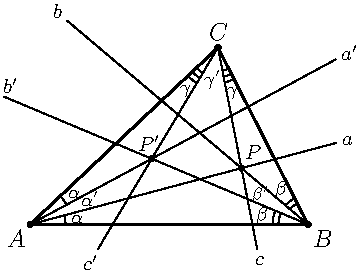
\includegraphics[width=87mm]{./img/theory/isogonal.pdf}}
	%\vspace{-1cm}
\end{wrapfigure}
\noindent\(\angle PBP' = \beta'\) (здесь все углы
ориентированные). Тогда для прямых  \(a, \, b, \, c\) из угловой теореме
Чевы имеем следующее:
\[
\frac{\sin \alpha}{\sin(\alpha + \alpha ')} \cdot
\frac{\sin(\gamma + \gamma ')}{\sin \gamma} \cdot
\frac{\sin \beta}{\sin(\beta + \beta ')} 
 = 1
\]

\noindent А теперь заметим, что 
\[
\frac{\sin(\alpha + \alpha ')}{\sin \alpha} \cdot
\frac{\sin \gamma}{\sin(\gamma + \gamma ')} \cdot
\frac{\sin(\beta + \beta ')}{\sin \beta} 
 = 1
\]
Но ведь это --- выражение угловой формы теоремы Чевы для прямых
\(a'\), \(b'\), \(c'\). А значит, согласно угловой теореме Чевы, 
\(a'\), \(b'\), \(c'\) проходят через \(P'\).
%\(a' \cap b' \cap c' = p'\).
%Обратное следствие доказывается аналогично. 
\end{proof} \vspace{-4mm} 

\begin{note}
Точки \(P\) и \(P'\) называют \textit{изогонально сопряжёнными} 
относительно \textbf{треугольника} \(ABC\), если они существуют, 
то есть если соответствующие прямые непараллельны.
%Отметим также, что в общем случае, то есть в случае, когда \(a\), \(b\) и \(c\) 
%могут быть вне треугольника \(ABC\), из конкурентности \(a\), \(b\) и \(c\) не 
%следует конкурентность \(a'\), \(b'\) и \(c'\), так как в угловую теорему Чевы 
%входят имеено \textit{ориентированные} углы, синусы которых меняются при 
%отражении относительно биссектрисы угла. \\
%что нам не пришлось отдельно разбирать
%случай, когда прямые \(a\), \(b\), \(c\) параллельны, так как это учтено в
%угловой теореме Чевы.\\
\end{note}

Используя данный метод, можно мгновенно получить, например, что высоты
пересекаются в одной точке. Для этого достаточно заметить, что 
\(\angle OAC = \angle H_aAB\), где \(AH_a\) --- высота в треугольнике \(ABC\).
То есть \(AH_a\) и \(AO\) --- изогонали относительно угла \(CAB\) треугольника
\(ABC\). Проведя аналогичные рассуждения для оставшихся двух высот и применив
к ним вышесформулированную теорему, получим требуемое.

Пересечение \textit{симедиан} в одной точке также доказывается в один ход, а
именно: медианы пересекаются в одной точке, а симедианы \textit{по определению}
симметричны медианам относительно биссектрис углов. Применяя теперь только что
доказанную теорему, получим искомое утверждение.\\

\noindent Приведем ниже, как дополнение, интересный факт,
доказательство которого вы можете найти, например, в статье
\textquote{Теорема об изогоналях} А.Куликовой и Д.Прокопенко.

%\noindent {\normalfont\fontsize{14}{14}\textbf{Теорема об изогоналях}}. 
\begin{theorem}
Пусть \(OB\) и \(OC\) --- изогонали угла \(AOD\). Прямые
\(AC\) и \(BD\) пересекаются в точке \(Q\), прямые \(AB\) и \(CD\)
--- в точке \(P\). Тогда \(OP\) и \(OQ\) --- также изогонали 
относительно угла \(AOD\).\\
\end{theorem}

\subsection{Изотомическое сопряжение}


\begin{definition}
Точки \(P\) и \(Q\) называются \textbf{изотомически сопряженными}
относитильно \textbf{отрезка} \(AB\), если они %лежат на прямой \(AB\) и 
симметричны относительно середины этого отрезка.\\
\end{definition}

\begin{theorem}
Пусть на прямых \(BC\), \(AC\), \(AB\), образующих треугольник \(ABC\),
отмечены точки \(A_1\), \(B_1\), \(C_1\) соответственно. Точки
\(A_2\), \(B_2\), \(C_2\) изотомически сопряжены точкам \(A_1\), \(B_1\), 
\(C_1\) относительно отрезков \(BC\), \(AC\), \(AB\) соответственно.
Тогда для того, чтобы прямые \(AA_1\), \(BB_1\), \(CC_1\) были конкурентны,
необходимо и достаточно, чтобы прямые \(AA_2\), \(BB_2\), \(CC_2\) были таковыми.
\end{theorem}


\begin{proof}
Докажем сначала, что из конкурентности прямых \(AA_1\), \(BB_1\), \(CC_1\)
следует конкурентность прямых \(AA_2\), \(BB_2\), \(CC_2\). 
%asddgsdg egewg wefew fwef wef ewfw    e efe    wf    wef     wef
%wefw    efw    efw    efwe    fewf wefwex    zqwwfhz    whnuw    h
%    WFN	efheuw    hfuhuI	HEFuhwfUwehfiuhf


По определению %\textit{изотомического сопряжения}
%точек относительно сторон треугольника \(ABC\)
имеем: \(\vecarrow{AB_2} = \vecarrow{B_1C_{\: \,}} = 
\vecarrow{x_{\,}}\), \(\vecarrow{CA_2} = \vecarrow{A_1B_{\;}} = 
\vecarrow{y_{\,}}\), \(\vecarrow{BC_1} = \vecarrow{C_2A_{\:}} =
\vecarrow{z_{\, \,}}\).
Положим \(\Overrightarrow{B_2B_1} = \vecarrow{x_1}\), \(\Overrightarrow{A_2A_1}
 = \vecarrow{y_1}\), \(\Overrightarrow{C_2C_1} = \vecarrow{z_1}\).


\begin{wrapfigure}{l}{87mm}
    \vspace{-0.7cm}
    \fcolorbox{white}{white}{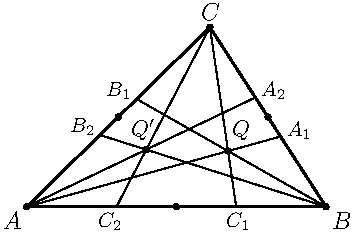
\includegraphics[width=87mm]{./img/theory/isotomic.pdf}}
	\vspace{-1cm}
\end{wrapfigure}


Тогда, применив теорему Чевы для прямых \(AA_1\), \(BB_1\), \(CC_1\),
получим:

\begin{ceqn}
\[
\frac{\vecarrow{x_{\,}} + \vecarrow{x_1}}{\vecarrow{x_{\,}}} \cdot
\frac{\vecarrow{y_{\,}} + \vecarrow{y_1}}{\vecarrow{y_{\,}}} \cdot
\frac{\vecarrow{z_{\, \,}} + \vecarrow{z_1}}{\vecarrow{z_{\, \,}}} 
= 1
\]
\end{ceqn}


Теперь заметим, что имеет место равенство 
\begin{ceqn}
\[
\frac{\vecarrow{x_{\,}}}{\vecarrow{x_{\,}} + \vecarrow{x_1}} \cdot
\frac{\vecarrow{y_{\,}}}{\vecarrow{y_{\,}} + \vecarrow{y_1}} \cdot
\frac{\vecarrow{z_{\, \,}}}{\vecarrow{z_{\, \,}} + \vecarrow{z_1}} 
= 1
\]
\end{ceqn}

А значит, согласно теореме Чевы, прямые \(AA_2\), \(BB_2\), \(CC_2\) конкурентны.
Следствие в обратную сторону доказывается аналогично.
%\lipsum[2-4]
\end{proof}


\begin{note}
Точки \(Q\) и \(Q'\) называются \textit{изотомически сопряженными} относительно 
\textbf{треугольника} \(ABC\), если они существуют, то есть если соответствующие
прямые непараллельны. Стоит отметить, что в отличие от \textit{изогонального 
сопряжения} точки \(A_1\), \(B_1\) и \(C_1\) не обязаны принадлежать сторонам 
треугольника \(ABC\), они могут лежать и вне их, на прямых, содержащие стороны 
треугольника \(ABC\).
%нам не пришлось отдельно разбирать
%случай, когда прямые \(AA_1\), \(BB_1\), \(CC_1\) параллельны, так как это
%учтено в теореме Чевы. 
\vspace{-4mm} \\
\end{note}

\begin{wrapfigure}{r}{70mm}
    \vspace{-0.45cm}
    \fcolorbox{white}{white}{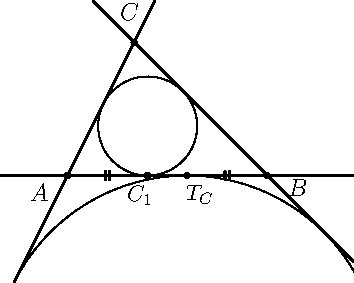
\includegraphics[width=70mm]{./img/theory/excircle.pdf}}
    %\fbox{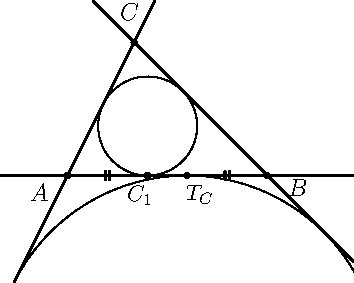
\includegraphics[width=70mm]{./img/theory/excircle.pdf}}
	%\vspace{-3cm}
\end{wrapfigure}


Несложно видеть, что точки касания вписанной и соответствующей вневписанной 
оружностей изотомически сопряжены относительно соответствующей стороны 
треугольника \(ABC\) (см. рис.). Тогда, проделывая аналогичные рассуждения
для всех сторон треугольника \(ABC\) и применяя только что доказанну 
теорему, получим, что точки Нагеля и 
Жергонна \textit{изотомически сопряжены}. \\

%\textbf{ТУТ БУДЕТ НАПИСАНО ПРО ИЗОТОМИЧЕСКОЕ СОПРЯЖЕНИЕ}\\
%\vspace{20mm}
\vspace{5mm}
%\noindent 

%%%
%Понятное дело, что это далеко не самый полный список методов
%доказательства подобного рода задач.
%Цель данного раздела --- показать, в каких
%направлениях можно начать действовать
%в задачах такого типа.

\section*{Примеры}
Давайте рассмотрим теперь применение данных методов при решение
конкретных задач. Примеры специально разбираются так подробно,
чтобы продемонстрировать решение задачи от идеи до полного, 
окончательного решения.\\

%\noindent \textbf{Пример 1}.
\begin{example}{1}
В треугольнике $ABC$ $AL_a$, $BL_b$, $CL_c$
--- биссектрисы, $K_a$ --- точка пересечения касательных к описанной
окружности в вершинах $B$ и $C$, $K_b$, $K_c$ определены
аналогично. Докажите, что прямые $K_a L_a$, $K_b L_b$ и $K_c L_c$
пересекаются в одной точке.
\textit{(Заочный тур oлимпиады им. И.Ф.Шарыгина 2019)}\\
\end{example}


%\hfill \break

\begin{solution}
    Чтобы понять, какой из вышеописанных методов поможет в решении
    данной задаче, обратимся к рисунку (см. рис. 1). 
	Из известных преобразований плоскости тут мало что может помочь.
	Действительно, используя, \textit{поворот}, или \textit{осевую симметрию},
	или \textit{параллельный перенос} --- не совсем понятно относительно
	чего производить
	эти преобразования, и что куда при них перейдет.
	\textit{Инверсия} здесь явно не поможет, потому что данные прямые не 
	проходят через центр какой-нибудь \textquote{\textit{удобной}} 
	окружности, и поэтому вообще перейдут в окружности, следовательно нам
	ничего доказать не удастся. 
    Использование \textit{гомотетии} также не 
	кажется, по крайней мере на первый взгляд, осмысленным, т.к.
	мы ничего не можем сказать про отношения отрезков 
	(кроме, разве что, в $\triangle ABC$), поэтому не поймем что куда 
	перейдет. Остается последний вариант --- теорема Чевы. На первый
	взгляд её использование здесь вам может показаться неуместным, но
	не торопитесь с выводами. Итак, давайте разбираться, как же
	все-таки здесь использовать теорему Чевы. 

	\begin{figure}[H]
	
	%\vspace{-1cm}
	\hspace{1cm}
	%\centering
	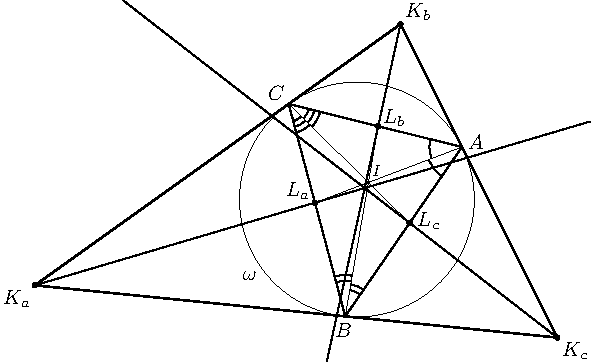
\includegraphics[width=15cm]{./img/examples/sharygin_19_2019.pdf}
	\caption{}
	\end{figure}

    Как мы помним, в теореме Чевы нам нужно, чтобы произведение отношений
	соответствующих направленных отрезков было равно 1, тогда и только тогда
	прямые пересекутся в одной точке. Здесь отношения таких отрезков 
	считать неудобно, поэтому давайте лучше постараемся
	все-таки понять что-то про расположение данных прямых. 
	Единственное, отношение чего мы знаем --- отношения отрезков, содержащие
	основания биссекрис $\triangle ABC$. Было бы хорошо понять что-нибудь 
	про расположение самих прямых, например, углы относительно сторон 
	$\triangle K_a K_b K_c$. Давайте отдельно перерисуем фрагмент рисунка, 
	содержащий одну из трех прямых ($K_a L_a$, $K_b L_b$, $K_c L_c$),
	и исследуем его.


	\begin{wrapfigure}{l}{8cm}
	
	\vspace{-1cm}
	%\hspace{6cm}
	%\centering
	\fcolorbox{white}{white}{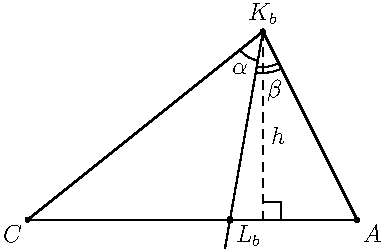
\includegraphics[width=8cm]{./img/examples/sharygin_19_2019_2.pdf}}
	%\caption{}
	\end{wrapfigure}

	{\setstretch{1.5} Попробуем что-то узнать про углы \(\alpha\)
    и \(\beta\), учитывая отношение $\dfrac{CL_b}{L_bA}$. 
	Давайте вспомним, что площадь треугольника
	можно посчитать как полупроизведение сторон на синус угла между ними.
	То есть \hspace{0mm} $S_{CK_bL_b} = \dfrac{CK_b 
	\cdot K_bL_b \cdot \sin \alpha}{2}$.
	Аналогично $S_{AK_bL_b} = \dfrac{K_bL_b \cdot K_bA \cdot \sin \beta}{2}$.
	Откуда получаем $\dfrac{S_{CK_bL_b}}{S_{AK_bL_b}} = \dfrac{CK_b \cdot
	\sin \alpha}{K_bA \cdot \sin \beta}$.
	С другой стороны 
	$S_{AK_bL_b} = \dfrac{h \cdot L_bA}{2}$ \hspace{0mm} и 
	\hspace{0mm} $S_{CK_bL_b} = \dfrac{h \cdot L_bC}{2}$. \par }
	
	{\setstretch{1.8} Тогда \hspace{0mm} $\dfrac{S_{CK_bL_b}}{S_{AK_bL_b}} = 
	\dfrac{L_bC}{L_bA}$. И окончательно $\dfrac{S_{CK_bL_b}}{S_{AK_bL_b}} =
	\dfrac{CK_b \cdot \sin \alpha}{K_bA \cdot \sin \beta} = 
	\dfrac{L_bC}{L_bA}$.
	
    Но ведь  $K_bC$ и $K_bA$ --- это отрезки касательных к
	окружности $\omega$ из одной \par} \noindent точки $\Rightarrow 
	K_bC = K_bA$. \\ \indent В итоге полученное выражение преобретает вид
	$\dfrac{\sin \alpha}{\sin \beta} = \dfrac{L_bC}{L_bA}$.

	Мы видим отношение двух синусов, что наталкивает нас на мысль о том, что
	на самом деле мы будем использовать \textit{угловую} форму
	теоремы Чевы.

	Теперь остается лишь написать схожее отношение для всех трех прямых 
	и перемножить.\\

    
	$\dfrac{\sin \angle K_cK_aL_a}{\sin \angle L_aK_aK_b} \cdot
	\dfrac{\sin \angle K_aK_bL_b} {\sin \angle L_bK_bK_c} \cdot
	\dfrac{\sin \angle K_bK_cL_c}{\sin \angle L_cK_cK_a} = 
	\dfrac{BL_a}{L_aC} \cdot \dfrac{CL_b}{L_bA} \cdot \dfrac{AL_c}{L_cB} = 1$ \\
	
	(последнее равенство верно, т.к. биссектрисы пересекаются в одной точке)

	Тогда, согласно \textquote{\textit{угловой}} форме теоремы Чевы,
	прямые $K_aL_a, K_bL_b, K_cL_c$ пересекаются в одной точке. 
    \textbf{\fontsize{13}{13}\selectfont Что и требовалось доказать.} \vspace{2mm}

\end{solution}


\begin{remark}
	Вектора мы опустили, потому что основания бисcектрис всегда лежат
	на сторонах треугольника.
	Однако стоит отметить, что условие \textquote{$BL_b, AL_a, CL_c$ 
	--- биссектрисы}
	мы использовали, только когда считали отношение синусов
	соответствующих углов. То есть, вообще-то говоря,
    $BL_b, AL_a, CL_c$ могли быть любыми \textit{чевианами} в $\triangle ABC$,
	основания которых лежат на сторонах треугольника,
    и которые  пересекаются в одной точке.\\
\end{remark}

\begin{example}{2}
В треугольнике $ABC$ $AH_1$ и $BH_2$ ---  высоты; касательная к описанной
окружности в точке $A$ пересекает $BC$ в точке $S_1$, а касательная в точке
$B$ пересекает $AC$ в точке $S_2$; $T_1$ и $T_2$ --- середины отрезков
$AS_1$ и $BS_2$. Докажите, что $T_1T_2$, $AB$ и $H_1H_2$
пересекаются в одной точке.
\textit{(Заочный тур oлимпиады им. И.Ф.Шарыгина 2019)}\\
\end{example}

\begin{solution}
На первый взгляд задача кажется достаточно трудной, однако можно снова
обратиться к списку вышеописанных методов и выбрать нам подходящий, 
как мы делали в предыдущем примере.\\
\end{solution}

\begin{example}{3}
Даны три окружности. Первая и вторая пересекаются в точках $A_0$ и $A_1$,
вторая и третья --- в точках $B_0$ и $B_1$, третья и первая --- в точках
$C_0$ и $C_1$. Пусть $O_{i,j,k}$ --- центр описанной окружности
треугольника $A_iB_jC_k$ . Через все пары точек	вида $O_{i,j,k}$
и $O_{1−i,1−j,1−k}$ провели прямые. Докажите, что эти 4 прямые пересекаются
в одной точке или параллельны.
\textit{(Заочный тур oлимпиады им. И.Ф.Шарыгина 2019)}\\
\end{example}

\begin{solution}
\end{solution}

\begin{example}{4}
Каждая из окружностей \(S_1\), \(S_2\) и \(S_3\) касается внешним образом
окружности \(S\) (в точках \(A_1\), \(B_1\), \(C_1\) соответственно) и двух
сторон треугольника \(ABC\) (см. рис.). Докажите, что прямые \(AA_1\),
\(BB_1\), \(CC_1\) пересекаются в одной точке. 
(\textit{Всеросс., 1994, финал, 10})
\end{example}

\begin{solution}
\end{solution}


\section*{Задачи}
ТУТ БУДУТ ЗАДАЧИ ДЛЯ САМОСТОЯТЕЛЬНОГО РЕШЕНИЯ.



\section*{Подсказки}
ТУТ БУДУТ ПОДСКАЗКИ К ЗАДАЧАМ ДЛЯ САМОСТОЯТЕЛЬНОГО РЕШЕНИЯ.




\begin{thebibliography}{9}
\bibitem{ponarin}
Я. П. Понарин Элементарная геометрия Том 1

\bibitem{kulikovaprokopenko}
А.Куликова, Д.Прокопенко --- \textquote{Теорема об изогоналях} \\
\texttt{http://geometry.ru/articles/isogonal\_theorem\_kvant\_04\_05.pdf}

\end{thebibliography}



\end{document}
